\chapter{Conversion A/N}
\section{Introduction}
La conversion A/N qui s'effectue au niveau de la carte d'acquisition est une opération de double quantification, recouvrant 2 problématiques:
\begin{itemize}
	\item discrétisation du temps ou \emph{échantillonnage} du signal, dont le paramètre principal est la \emph{fréquence d'échantillonnage}, est réalisé par un convertisseur A/N (CAN ou ADC) ou par un circuit spécifique nommé "échantillonneur-bloqueur" (sample \& hold ou S \& H)
	\item la discrétisation en amplitude ou \emph{quantification}, dont le principal paramètre est le \emph{nombre de bits} du convertisseur A/N (2\up{N} niveaux pour un convertisseur à N bits)
\end{itemize}
\begin{figure}[H] 
	\centering 
	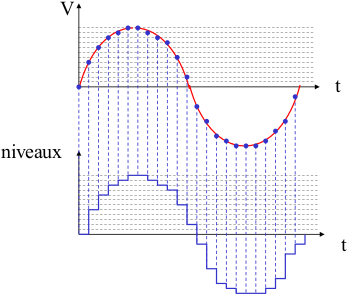
\includegraphics[width=0.8\textwidth,height=10\baselineskip,keepaspectratio]{ch5/image1} 
	\caption{Conversion A/N}
	\label{fig:conversionan} 
\end{figure}
\section{Échantillonnage (S \& H)}
\subsection{Repliement spectral (aliasing)}
On commence par le problème de quantification temporelle. Le choix de la fréquence d'échantillonnage est crucial. En effet, si la fréquence d'échantillonnage est trop faible, alors nous ne pourrons pas retrouver notre signal initial  car le nombre d'échantillons par période est trop faible (\textit{C.f.} \autoref{fig:replispectral}). C'est le repliement spectral.
\begin{figure}[H] 
	\centering 
	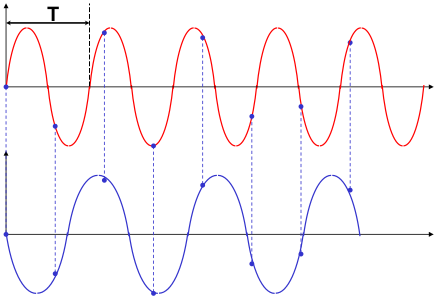
\includegraphics[width=0.8\textwidth,height=10\baselineskip,keepaspectratio]{ch5/image2} 
	\caption{Repliement spectral} 
	\label{fig:replispectral}
\end{figure}
\subsection{Fréquence d'échantillonnage}
Pour choisir notre fréquence d'échantillonnage, on aura recours au Critère de Nyquist
\[f_s>2f_{max}\quad\text{où}\quad \left\{\begin{array}{ll}
f_s &= \text{fréquence d'échantillonnage (sampling)}\\
f_{max} &= \text{fréquence maximale contenue dans le signa}
\end{array}\right.\]
Ceci est une condition nécessaire (donc NON suffisante). La plupart du temps, il faudra prendre \(10\times f_{max}\) pour avoir une bonne précision. Il faut typiquement, 7 à 10 échantillons/période pour une bonne précision.\\
Si ce critère n'est pas respectée \(\Rightarrow\) Repliement spectral.
\paragraph{Remarque:} On serait tenté de se dire "Je ne veux pas numériser des fréquences plus élevées de mon signal analogique car elles ne m'intéresse pas, donc je ne vais pas les prendre en compte pour le critère et elles seront donc éliminer". Grave erreur. Le principe du repliement spectral est que les fréquence plus élevée que \(\frac{f_s}{2}\) seront ramenées à des fréquences plus basses, et donc viendront dégrader notre signal. Pour éviter cela, il faut impérativement mettre un filtre passe-bas "anti-repliement" AVANT le convertisseur afin d'éliminer les hautes fréquences (les fréquences qu'on ne voulait pas) et donc rendre l'effet de leurs repliements négligeable par rapport au signal.
\subsection{Temps et erreur d'ouverture (sample \& hold)}
Une fois qu'on a choisi notre fréquence d'échantillonnage, on a un autre problème: pour quantifier le signal analogique en valeur numérique, il faut que l'amplitude du signal analogique ne varie pas (ou pas trop).\\
On définit donc l'\emph{ouverture} ou la \emph{durée d'ouverture} \(t_A\) (aperture time) la durée durant laquelle un signal analogique (échantillon) doit être présenté à l'entrée de CAN afin qu'il puisse le convertir en valeur numérique.\\
Il est probable que le signal varie durant cette période, auquel cas il y aura un risque de dégrader la précision de la conversion. L'erreur d'ouverture (absolue) vaut \((\text{dérivée max du signal})\times t_A\)\\

\danger La durée d'ouverture n'est ni la période d'échantillonnage (temps entre 2 échantillons), ni le temps de conversion (durée nécessaire au CAN pour convertir un échantillon).\\

Si \(t_A\) est trop grand par rapport à l'erreur de tolérable, on peut:
\begin{itemize}
	\item changer d'ADC avec un \(t_A\) plus faible mais qui coûtera sûrement plus cher
	\item ajouter un circuit sample \& hold avant l'ADC (moins coûteux, préféré).
\end{itemize}
Le circuit sample \& hold aura pour fonction d'échantillonner le signal analogique très rapidement (\(t_A\) faible) afin de présenter en sortie une valeur analogique constante pendant toute la période d'échantillonnage (l'ADC pourra faire la conversion à l'aise). En résumé, il transforme un signal analogique continu en palier mais sans quantifier l'amplitude.
\section{Quantification (CAN)}
\subsection{Principe}
Le CAN transforme une tension analogique constante (échantillon) en un code numérique sur N bits, défini en fonction de la résolution voulue.\\
On définit le LSB, le "Least Significant Bit" ou le bit de poids le plus faible, utilisé comme unité de mesure car il représente le pas de quantification du signal analogique. Sachant que FSR = full scale range (la plage des valeurs possible, genre pour un \SI{+-5}{\volt}, c'est \SI{10}{\volt}), on a
\[1\,LSB = \left\{\begin{array}{lc}
FSR/2^{N}\\
FSR/(2^N-1) & \text{si premier et dernier échellon = demi-intervalle}
\end{array}\right.\]
Il faudra faire un compromis entre rapidité de conversion de l'ADC et sa résolution.
\subsection{Caractéristique d'un CAN idéal}
\begin{figure}[H] 
	\centering 
	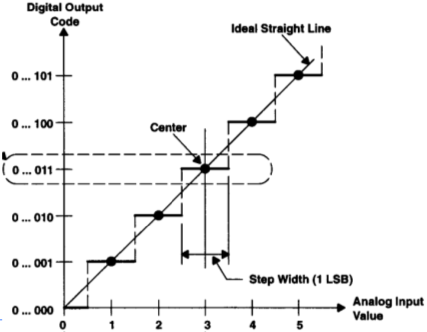
\includegraphics[width=0.8\textwidth,height=10\baselineskip,keepaspectratio]{ch5/image3} 
	\caption{CAN idéal} 
\end{figure}
la résolution est définie comme la plus petite différence détectable, donc 1 LSB\\
Dans un CAN idéal, nous n'avons que l'erreur de quantification:
\begin{itemize}
	\item due à la conversion d'un signal continu en un signal quantifié (inhérent au CAN)
	\item valant \(\pm 1/2\,LSB\)
\end{itemize}
Des exemples de valeurs sont représentés \autoref{fig:exvaladc}
\begin{figure}[H] 
	\centering 
	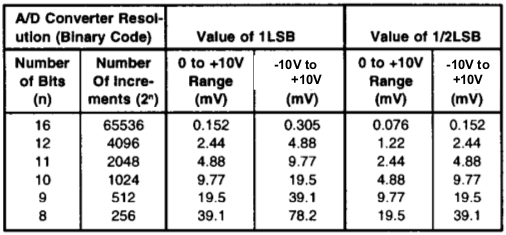
\includegraphics[width=0.8\textwidth,height=10\baselineskip,keepaspectratio]{ch5/image4} 
	\caption{Exemples de résolutions et d'erreur de quantification}
	\label{fig:exvaladc} 
\end{figure}
\subsection{Autres sources d'erreur d'un CAN réel}
Dans un CAN réel, on a un peut plus de source d'erreur:
\begin{itemize}
	\item erreur de décalage ou offset error (ne passe pas par 0)
	\begin{itemize}
		\item décalage horizontal de la caract.
		\item peut être compenser par calibration
	\end{itemize}
	\item erreur de gain ou gain error
	\begin{itemize}
		\item erreur sur la pente de la caract.
		\item peut être compensé par calibration
	\end{itemize}
	\item erreur de linéarité intégrale
	\begin{itemize}
		\item décalage horizontal restant (pour chaque pas) après avoir compensé les erreurs d'offset et de gain.
	\end{itemize}
	\item erreur de linéarité différentiel (erreur entre 2 codes successifs)
	\begin{itemize}
		\item erreur sur la largeur d'un palier
		\item peut mener à des codes manquants
	\end{itemize}
\end{itemize}
Ordre de grandeur de ces erreurs ? On fait la \(\sum\) quadratique des erreurs \(\Rightarrow\) ordre total comparable à celui de l'erreur de quantification.
\subsection{Propriétés diverses}
\begin{itemize}
	\item durée d'ouverture \(\rightarrow\) faut-il un sample \& hold?
	\item délai de conversion \(\rightarrow\ < 1/f_s\)
	\item type de codage numérique en sortie
	\begin{itemize}
		\item binaire
		\begin{itemize}
			\item unipolaire
			\item bipolaire avec offset
			\item bipolaire en complément à 2 
		\end{itemize}
		\item BCD (binary-coded-decimal)
		\begin{itemize}
			\item unipolar BCD
			\item sign-magnitude BCD
		\end{itemize}
	\end{itemize}
\end{itemize}
\subsection{Type de convertisseurs A/N}
\textit{C.f.} Wikipedia pour de plus amples explications dessus.
\subsubsection{À approximation successives (SAR)}
C'est une recherche dichotomique: charge un capa et lis la tension obtenue (recharge rapide) et recommence du MSB vers le LSB. Il a jusqu'à 16 bits de résolution (aujourd'hui 24), un faible temps de conversion. Bon pour du multiplexage
\subsubsection{Sigma-delta}
C'est une recherche en boucle fermée. Jusqu'à 24 vits de résolution, erreur linéaire différentielle très faible, temps de conversion élevé. Pas bon pour multiplexage
\subsubsection{ADC rapides}
Ils sont rapides mais moins précis. FLASH, subranging ou pipelined\bigskip